\documentclass[11pt,a4paper]{report}
\usepackage[utf8]{inputenc}
\usepackage{amsmath}
\usepackage{amsfonts}
\usepackage{amssymb}
\usepackage{graphicx}
\author{Ryan Lance}
\title{HWK 1}
\begin{document}

\paragraph{Capstones: Classical Mechanics, HWK 1.} Ryan Lance
\paragraph{Problem 1} A cannon shoots a ball with elevation angle (the angle from the horizontal) $\theta$ and initial speed $v_o$. Ignoring air friction, find the equation of motion of the ball in the horizontal direction $(x(t))$, in the vertical direction $(y(t))$, and eliminate time to find $y(x)$. Assume that the size of the cannonball is negligible.
\paragraph{Solution} Below is a picture of the problem. One assumption is that we are only concerned with the trajectory of the cannonball immediately after it leaves the barrel of the cannon, which is stationed at $(x_o, y_o)$. The cannon is angled at angle theta with respect to the ground, and the velocity of the cannonball as it leaves the cannon is $v_o$. 
\begin{center}
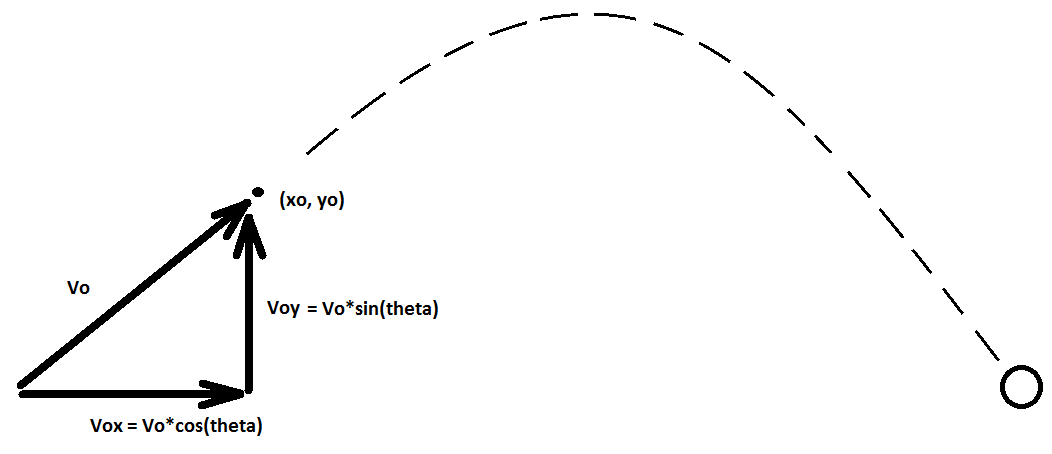
\includegraphics[scale=0.4]{projectile}
\end{center}
\paragraph{} We can start by splitting our velocity vector into two components $V_{ox}$ and $V_{oy}$ using sine and cosine. This way we can describe the horizontal and vertical components independently. Since our vertical axis is aligned with the gravitational field, and the cannonball is likely not going to travel very high or far, we can assume that the acceleration in the y-axis is a constant $g$ equal to $-9.81m/s^2$ and that the horizontal component of the acceleration is zero (because there is no drag). 

\paragraph{}First, we write down the acceleration component wise, then integrate with respect to time to find to find functions for velocity and position. The constants of integration become $v_{ox}, v_{oy}, x_o,$ and $y_o$.
\begin{center}
\begin{tabular}{l l}
$a_x(t) = 0$ 				& $a_y(t) = g$ \\
$v_x(t) = v_{ox}$ 			& $v_y(t) = gt + v_{oy}$ \\
$x(t) = v_{ox}t + x_o$ 		& $y(t) = 0.5gt^2 + v_{oy}t + y_o$ \\
\end{tabular}
\end{center}
\paragraph{}We now have equations for $x(t)$ and $y(t)$, but they are not in terms of $v_o$ and $\theta$. Substituting the following from earlier: $v_{ox} = v_osin\theta, v_{oy} = v_ocos\theta$, and set $x_o = y_o = 0$. 
\begin{center}
\begin{tabular}{l}
$x(t) = v_ocos\theta t$ \\ $y(t) = 0.5gt^2 + v_osin\theta t$ \\
\end{tabular}
\end{center}
\paragraph{}Solving for $t$ (now $x(t) = x$), we get a formula for time in terms of $x$:
$$t = \frac{x}{v_ocos\theta}$$
\paragraph{}Substituting this into our equation describing vertical motion $(y(t))$ we get a new function $y(x)$ that we were looking for:
$$y(x) = 0.5g(\frac{x}{v_ocos\theta})^2 + v_osin\theta(\frac{x}{v_ocos\theta})$$
\paragraph{}Simplification:
$$y(x) = \frac{gx^2}{2(v_ocos\theta)^2} + xtan\theta$$
\paragraph{Physical Reasoning} My physical intuition tells me that for some $\theta$ between $0$ and $\pi/2$, the motion should be a downward parabola beginning at $(x_o, y_o)$ (which is $(0, 0)$ in this case). Our solution takes the form: $ax^2 + bx$ where $a$ is negative because $g$ is negative and the denominator is squared. If we just look at $a$, we can see that it represents how quickly the trajectory will lead the cannonball back to $y = 0$. $a$ scales up with $g$ and it scales down with $v_o$. This makes sense because lower gravity or a larger initial velocity will shoot the cannonball higher and farther. Looking at the coefficient to the linear component, $tan\theta$, we see that at $\theta = 0$ the cannonball goes nowhere. When $\theta$ gets closer to $pi/2$ however, $tan\theta$ is much larger. This makes the parabola very "spiky", the cannonball is just shot up and straight down. Interestingly, this term also makes sense because when $\theta$ does go to $\pi/2$, the solution is undefined (a vertical line), which is what we expect the cannonball's path to be if the cannon is pointing straight up.

\paragraph{Problem 2} A brick, starting from rest, slides down an incline with kinetic friction coefficient $u_k$. Find the velocity of the brick when it hits the ground as a function of the angle $\theta$ that the plane makes with the horizontal and of the initial elevation $h$ of the brick from the ground. How much energy was dissipated into heat? Assume that the size of the brick is negligible.

\paragraph{Solution}We start with a diagram of problem that shows the brick resting on the slope at height h. The slope is making some angle $\theta$ with the ground.
\begin{center}
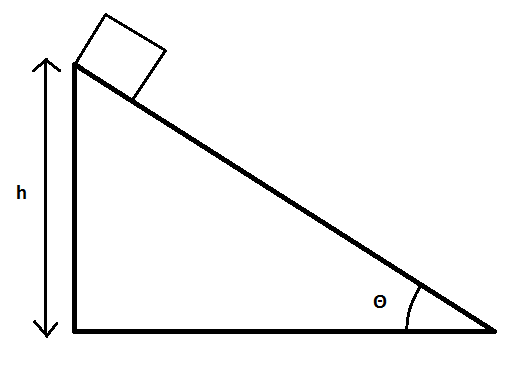
\includegraphics[scale=0.5]{ramp}
\end{center}
\paragraph{}Now we should use a free body diagram to determine the resulting motion of the brick. There appear to be only two forces acting of the brick at $t = 0$: the normal force of the slope holding the brick above the ground, and the force of gravity pulling the brick down. We will align our coordinate system so that down the slope is the positive x direction, the positive y direction is parallel to the normal vector of the face of the slope on which the brick is resting. 
\begin{center}
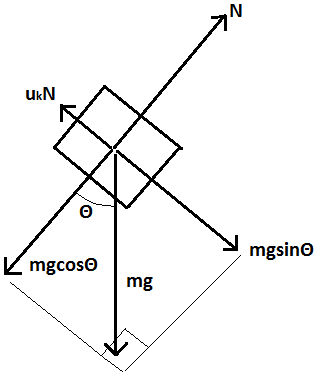
\includegraphics[scale=0.5]{FBD}
\end{center}
\paragraph{}The force of gravity acting on the brick is the gravitational constant at the Earth's surface ($g = -9.81m/s^2$) times the mass of the brick. This vector can then be split into it's constituent components according to our coordinate system.
\begin{center}
$F_{grav} = mgsin\theta\hat{x} + mgcos\theta\hat{y}$
\end{center}
\paragraph{}We can now sum the forces (the normal force and y component of gravitational force) in the y direction and set them equal to zero, then solve for the normal force.
\begin{center}
$\Sigma{\vec{F_y}} = ma_y$ \\
$N = mgcos\theta$
\end{center}
\paragraph{}We can set them equal to zero because we do not expect the block to accelerate in the y-direction. The normal force will only push as hard as it needs to hold up the brick. Now we do the same for the x component forces (friction and the component of gravity pointing down the slope).
\begin{center}
$\Sigma{\vec{F_x}} = ma_x$\\
$mgsin\theta - \mu_kN = ma_x$
\end{center}
\paragraph{}Substituting the normal force from earlier and solving for $a_x$ we obtain the following:
\begin{center}
$a_x = g(sin\theta - \mu_kcos\theta)$
\end{center}
\paragraph{}This solution makes sense in the case where $\theta$ is large enough to make the block slip. That is, when $F_{grav, x} > F_{friction}$ or $mgsin\theta > \mu_kN$. For angles where the force of gravity pulling the block down the slop does not overcome the frictional force, then acceleration will be zero. This can be writen as: 
\[
 a_x(t) = 
 \Big \{
 \begin{tabular}{l l}
  $0$ & $ sin\theta \leq \mu_kcos\theta$ \\
  $g(sin\theta - \mu_kcos\theta) $ & $ sin\theta > \mu_kcos\theta$ 
 \end{tabular}
\]
\paragraph{}Integrating we find the equations for position and velocity. Recall, the block starts from rest at the origin so we set the integration constant $v_{ox}$ and $x_o$ to $0$.
\[
 v_x(t) = 
 \Big \{
 \begin{tabular}{l l}
  $0$ & $ sin\theta \leq \mu_kcos\theta$ \\
  $g(sin\theta - \mu_kcos\theta)t $ & $ sin\theta > \mu_kcos\theta$ \\
 \end{tabular}
\]
\[
 x(t) = 
 \Big \{
 \begin{tabular}{l l}
  $0$ & $ sin\theta \leq \mu_kcos\theta$ \\
  $\frac{1}{2}g(sin\theta - \mu_kcos\theta)t^2 $ & $ sin\theta > \mu_kcos\theta$ \\
 \end{tabular}
\]
\paragraph{}The distance the block needs to travel in the x-direction is found by the trigonometric relationship between the ramp length, the initial height of the block and the angle of the ramp.
%\includegraphics[scale=0.5]{triangle with d, h and theta}
\begin{center}
$d = h/sin\theta$
\end{center}
If we let $x(t) = d$ we can find the time at which the block hits the ground.
\begin{center}
$\frac{1}{2}g(sin\theta - \mu_kcos\theta)t^2 = \dfrac{h}{sin\theta}$ \end{center}
Solving for time:
\begin{center}
$t_{bottom} = \sqrt{\dfrac{2h}{gsin\theta(sin\theta - \mu_kcos\theta)}}$
\end{center}
\paragraph{}Finally, we put this equation for time into our $v_x(t)$ function to obtain the velocity reached at the bottom of the slope.
\begin{center}
$v_x(t_{bottom}) = g(sin\theta - u_kcos\theta)\sqrt{\dfrac{2h}{gsin\theta(sin\theta - \mu_kcos\theta)}}$
\end{center}
Simplifying:
\begin{center}
$v_x(t_{bottom}) = \sqrt{\dfrac{2hg(sin\theta - \mu_kcos\theta)}{sin\theta}}$
\end{center}
\paragraph{}Solving for energy dissipated is just a matter of integrating the friction force over the distance travelled. Friction is not a function of position so our integration simplifies to multiplication.
\begin{center}
$\Delta E = F_{friction}\Delta x$ \\
$\Delta E = \mu_kmgcos\theta d$
\end{center}
\paragraph{Physical Reasoning}There are a few parts that we should analyze for physical reasoning. First is our derived formula for acceleration. The acceleration follows my physical intuition for the following reasons: First, when the coefficient of friction is zero, the solution is reduced to the frictionless slope solution $gsin\theta$. The next part is that as the angle of the slope increases, the acceleration in the x direction should increase, which it does. As $\theta$ increases, the term $sin\theta$ grows and the fritional component $\mu_kcos\theta$ shrinks. This means that friction plays less of a role at steeper angles. 
\paragraph{}The next piece we can analyze is the velocity of the brick at the bottom of the slope. There are more pieces to this, but the angle of the slope plays the same role. As it increases, the term$(sin\theta-\mu_kcos\theta)/sin\theta$ also increases as it did for acceleration. The height and strength of gravity also increase the speed at the bottom as expected.

\end{document}
